\section{Experimental Setup}
\label{sec:exp-setup}

\cmtDK[inline]{15 pages}

In this section I will describe which experiments were conducted to answer the \cmtDK{?}{questions} from the previous sections as well as the setup of these experiments.
This will be done in two parts.
The first part contains the creation of the datasets that will be used in the experiments.
In the second part I will go deeper into discussing each experiment, including the necessity of the experiment, the specifities of the dataset, as well as the final architecture of the models.

\subsection{Creation of the dataset}
The basis for my datasets is the CLEVR dataset (\cite{Johnson2016}).
This dataset includes 3D-generated images depicting scenes with different kinds of objects.
Each of these objects has different combinations attributes, such as \emph{shape}, \emph{color}, \emph{size} and \emph{material}.
The possible values of these attributes are listed in Table \ref{tab:clevr-attributes}.
Three to ten objects are randomly placed into the scene and assigned with random attributes.
To enhance realism and reduce ambiguity, objects do not intersect, have a certain distance from each other, and are at least partially visible.
Figure \ref{fig:clevr-example} shows an example of a generated image in the CLEVR dataset.

\begin{table}[h]
    \centering
    \begin{tabular}{cccc}
        \toprule
        \textbf{ shape } & \textbf{ color } & \textbf{ size } & \textbf{ material } \\
        cube             & gray             & small           & rubber              \\
        sphere           & red              & large           & metal               \\
        cylinder         & blue                                                     \\
                         & green                                                    \\
                         & brown                                                    \\
                         & purple                                                   \\
                         & cyan                                                     \\
                         & yellow                                                   \\
        \bottomrule
    \end{tabular}
    \caption{Attributes of objects in the CLEVR dataset}
    \label{tab:clevr-attributes}
\end{table}

\begin{figure}[h]
    \centering
    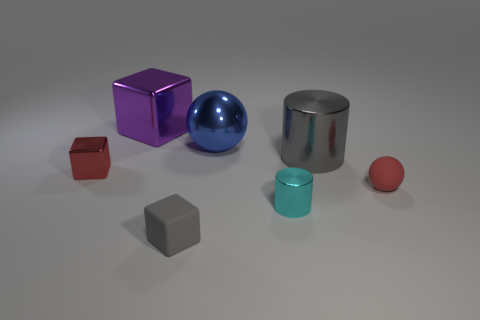
\includegraphics[width=.8\linewidth]{figures/CLEVR_example.png}
    \caption{Example of a generated image in the CLEVR dataset}
    \label{fig:clevr-example}
\end{figure}

Furthermore, the dataset contains information about each scene.
This includes all selected attributes for each object as well as the exact position of the centers of all the objects, both 3D-coordinates in the 3D scene and 2D-coordinates in the final rendered image.
In addition, simple spatial relations (in front of, behind, left, right) between the objects are calculated and stored.
These are simply based on the 3D-coordinates of the objects in relation to the position of the camera.

\cmtDK[inline]{ambiguity}

This research investigates how agents communicate about the relations of objects seen in images.
For that reason, the original CLEVR dataset offers too little control over how the objects are created and in which relation they stand to each other.
Following, I extended the source code to generate images for the CLEVR dataset.\footnote{\href{https://github.com/DominikKuenkele/MLT\_Master-Thesis\_clevr-dataset-gen}{https://github.com/DominikKuenkele/MLT\_Master-Thesis\_clevr-dataset-gen}}
To simplify the generation and the later learning of the models, I only focused on the attributes with a high impact on the appearance of the object, namely the \emph{shape}, \emph{size} and \emph{color}.
The \emph{material} is always the same for all objects in a generated image.
There were three main extensions to the code:

First, objects in the scene were separated into three categories: one \emph{target object}, objects in a \emph{target group} and \emph{distractor} objects.
The target object is the main object in the scene that should be identified and communicated by the agents.
All other objects and their relations are based on this target object.
The target group contains similar objects to the target object.
These are objects that the agents need to discriminate the target object from.
Finally, the distractors are objects that add noise to the scene and should make it more complex. They expected to teach the agents more precise descriptions of the target object.
The number of the objects in both group can be controlled.

In a second step, when generating the images it is possible to define the relations between \emph{target object}/\emph{target group} and \emph{target object}/\emph{distractors}.
The relation is defined as \textbf{how many} attributes of the target object are identical with the attributes of a single object in the target group and distractors respectively.
For example the target object is a \emph{small red cube}.
If two attributes are shared between target object and target group, objects in the target group could include \emph{small blue cube}, \emph{big red cube} or \emph{small red sphere}, but couldn't include another \emph{small red cube} or a \emph{small blue cylinder}.
The number of shared attributes can also be set to a range to make the discrimination task more challenging.

Lastly, it is also possible to define exactly \textbf{which} attributes should be shared between the target object and the groups.
For example, it can be defined to have the same size for objects in the target group, but have different, randomly selected shapes and colors.
This allows for a very controlled generation of relations between the objects in the scene.
Figure \ref{fig:clevr-extended_example} shows one generated image with this extended source code.
Here, the target object is the large purple cylinder.
The target group contains four objects that share zero to a maximum of two attributes.
It is not controlled, which attributes are shared (they are selected randomly). The large purple cylinder shares the same color and size with the large purple spherem, the same size with both cubes and no attribute with the small turquoise sphere.
There are no distractor objects.

\begin{figure}[h]
    \centering
    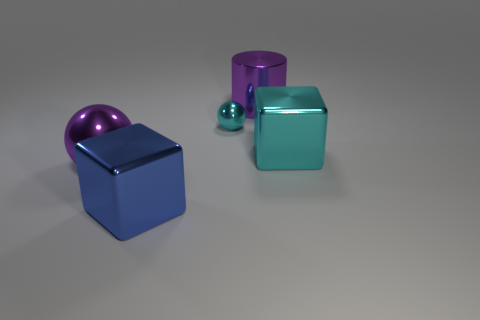
\includegraphics[width=.8\linewidth]{figures/CLEVR_extended_example.png}
    \caption{Example of a generated image with the extended code}
    \label{fig:clevr-extended_example}
\end{figure}

For all generated datasets in the following sections, the general constraints and settings are as close as possible to the original CLEVR dataset.
The size of the generated images is 480x320 pixels.
10.000 images are created for each of the datasets.
Each image contains a maximum of 10 objects, that are not intersecting, have the same minimum distance between objects and are partially visible from the camera.

\subsection{Description of experiments}
Language games are very complex setups for machine learning models.
The models need to solve multiple tasks at the same time to solve the overall problem.
For instance, in a simple setup of a game two agents are involved.
The first agent, the sender, is shown a scene with objects and needs to communicate one target object to the other agent, the receiver.
The receiver is shown the same scene and needs to identify the target object with respect to the message of the sender.
In this case, the sender first needs to learn to encode the scene, all objects and their attributes, as well as the information about the target object into its own \cmtDK{?}{space}.
In a next step it needs to learn how to translate this encoding into a message that is sent to the receiver.
The receiver then needs to learn to decode this message, after which it needs to learn how to combine the decoded message with its own encoding of the scene and objects.
And finally it needs to learn how to identify the target object with this information.

For this reason, I decided to divide the main problem and let the models learn simpler subtasks and increase the complexity step by step.
This will give me a very detailed overview, where the models struggle to learn and in which ways they can be improved.
Mainly, I separated the tasks into language games with two agents (final experiments) and classical machine learning tasks without any communication, namely only one 'agent' that solves the task alone (pre-experiments).
With this division, I can analyze the learning of the encodings of the scenes separately from the learning of producing and decoding messages.

\subsubsection{Feature extractors}
To extract features from the images, I make use of different deep neural network architectures that are developed for this task.
First, I use the \cmtDK{why ResNet/VGG?} VGG19 (\cite{Simonyan2015}) which is an architecture based on many convolutional layers.
After the convolutional layers, the data is passed first through an average pooling layer which outputs 512x7x7 dimensions.
Next follow three linear layers with \emph{ReLU} non-linearities in between.
After flattening the input, these classification layers output 4069, 4069 and 1000 dimensions respectively.

Secondly, I include the ResNet-101 (\cite{He2016}) that tries to overcome problems of very deep networks, using \cmtDK{needs to be explained deeper?}{residual blocks}.
There are four blocks that output 256x56x56, 512x28x28, 1024x14x14 and 2048x1x1 dimensions.
A following average pooling layer outputs 2048x1x1 dimensions as well.
The final linear layer reduces the flattened data to 1000 dimensions, corresponding to the ImageNet classes.

Both architectures are available pretrained on an image classification task on the ImageNet dataset.
Since the task in this research is very different from a classification, multiple different adaptions of these architectures are compared. \cmtDK{deeper discussion about different layers of these networks}
Table \ref*{tab:feature-extractor-archs} lists the different adaptions for both VGG19 and ResNet-101 that will be used in this research.
In the later chapters, it will be referred to these adaptions using the name in the table.

\begin{table}[h]
    \centering
    \begin{tabular}{rlc}
        \toprule
                            & \textbf{description}                                            & \textbf{ output dimensions } \\\midrule
        \textbf{VGG-0}      & contains only the convolutional layers                          & 512x7x7                      \\
        \textbf{VGG-avg}    & contains an additional average pooling layer                    & 512x7x7                      \\
        \textbf{VGG-cls1}   & \makecell[cl]{contains an additional one classification layer,                                 \\ including its non-linearity} & 4069                         \\
        \textbf{VGG-cls2}   & \makecell[cl]{contains another additional classification layer,                                \\ including its non-linearity} & 4069                         \\
        \textbf{VGG-cls3}   & the original VGG19 architecture                                 & 1000                         \\\midrule
        \textbf{ResNet-1}   & contains one residual block                                     & 256x56x56                    \\
        \textbf{ResNet-2}   & contains two residual blocks                                    & 512x28x28                    \\
        \textbf{ResNet-3}   & contains three residual blocks                                  & 1024x14x14                   \\
        \textbf{ResNet-4}   & contains four residual blocks                                   & 2048x1x1                     \\
        \textbf{ResNet-avg} & contains an additional average pooling layer                    & 2048x1x1                     \\
        \textbf{ResNet-cls} & the original ResNet-101 architecture                            & 1000                         \\
        \bottomrule
    \end{tabular}
    \caption{Different adaptions of VGG19 and ResNet-101 used in this research}
    \label{tab:feature-extractor-archs}
\end{table}

Furthermore, I experimented with both the pretrained models as well as with the architectures trained from scratch with a random initialization for the weights.
This reason for this was to test if the success of an experiment was actually making use of the pretrained knowledge incorporated in the models.
If that was not the case, the agents were likely not using image features, but instead relying on some other underlying patterns to solve the task.
Basically, this approach works as an indicator to determine the actual success of the agents aside from measures as the accuracy or precision.


\subsubsection{Pre-experiments without language games}
The final objective of this thesis is to find out, how agents can communicate about relations of objects spatially as well as based on their attributes.
Because of that, the first experiments focus on extracting information from images and combining them with structured knowledge.
Here, I structured the experiments into three levels.
In the first level, the model are trained to learn the position of objects in the image and attend to specific regions of the image.
In the second level, the models are trained to differentiate objects in the scene from each other.
The last level adds language to the experiment, more specifically the models learn to caption and describe objects in the image.
These combined experiments should lay the basis for how to build up the agents in the language games.

\paragraph{Level 1 - coordinate predictor:}

This level should help to analyze, how the final task of the language game should look like, in especially what the receiver is tasked to predict.
As described before, the sender should communicate an object in the image and the receiver needs to identify it.
The challenge lies in how the receiver refers to the identified object.
There are multiple possibilities, how it can be done.
One of them could be to describe the target object with human language, using the attributes.
The main goal however is to let the language of the agents emerge as natural as possible.
Including human knowledge into the task would bias also the emerged language towards attributes and words, humans are using.
For this reason, the final task of the receiver will be to 'point' to the target object.
Since also positional information of the objects should be part of the discrimination, the image will not be separated into several bounding boxes around the objects, but instead the whole image is the basis.
The models are therefore tasked to predict the center coordinates of the target object.
With this approach, the models receive few human knowledge, but are still able to rely on all information present in the image to discriminate the objects.

To achieve this goal, multiple setups of models are tested.
In the simplest setup, the model receives only the image \cmtDK{preprocess image} as an input and produces two numbers as an output, the predicted x- and y-coordinate of the target object.
Here the image is first passed through one of the \emph{feature extractors}.
Next, the extracted feature vector is flattened and passed through two linear layers with a \emph{ReLU} non-linearity between.
These reduce the dimensions first to 1024 and finally to 2.

To determine the loss, the euclidean distance between the resulting predicted point on the image and the ground truth point are calculated.
This distance is learned to be minimized.
By doing that, the model learns to focus and attend on a specific part in the image, in a perfect model the center of the target object.

With this simple setup, the model is in theory able to focus on an object in the image.
The problem arises as soon as multiple objects are present in the image.
There is no information available for the model to understand which one of these objects is the actual target object, except for the final calculation of the loss.
Since there is not necessarily a pattern for which object in the image is the correct target object over the whole dataset, the models will likely fail to generalize. \cmtDK{go deeper, why}
Therefore, the models need to receive more information.
Here, I try out four different ways to encode the target object.

In the first method, I encode the attributes of the target object as \textbf{one-hot encodings}.
There is a three-dimensional vector encoding the \emph{shape}, an eight-dimensional vector encoding the color and a two-dimensional vector encoding the two different sizes.
The dimensions of these vectors can either be zero or one, depending on the attributes of the target object.
These three encodings of the attributes are then concatenated.
The image is again passed through a feature extractor, before the flattened vector is reduced to 2048 dimensions with a linear layer.
The result is concatenated with the encoded attributes and passed to a final linear layer to predict the coordinates.

In an extension to this method, I also include the \textbf{center coordinates of all objects} in the image.
This should help the model to identify all possible options to chose from, when predicting the target object.
All the center coordinates are simply extracted and shuffled.
Since there are varying numbers of objects in the image, this vector of variable length is padded to 10 objects, resulting in a vector with a length of 20.
The padding objects have zeros for both coordinates, which no other real object can have.
For this model, I also made use of a more complex way to encode the image.
Here, I based the approach on code that implements baselines for the CLEVR dataset (\cite{Johnson2017}). \cmtDK{why?}
The image is first passed through the feature extractor.
Afterwards, a 2-dimensional convolutional layer, reduces the channels from 2048 to 512 channels with a kernel size of 1.
After applying the \emph{ReLU} function, the resulting matrix is max pooled over two dimensions with both a kernel size and a stride of 2.
The resulting matrix is flattened and concatenated with both the attribute encodings and the shuffled coordinates of all objects.
This is then passed again through a final linear layer to predict x- and y-coordinates.

The third method encodes the attributes of the target object with human language using the \textbf{incremental algorithm for the Generation of Referring Expressions (GRE)} described in \cite{Dale1995}.
This opposes the idea described before, to share as few human knowledge as possible with the model.
Still, this approach can help to understand and analyze if the model was able to extract information about the objects and more specifically their attributes from the image.
If the model is able to match parts of the image with human words it would show that the model learned this attribute.
If the model in a next step can learn this over the whole dataset, this would mean that it could generalize over these attributes and assign them to certain regions in an image.
This insight could help then to design another model that makes use of these learnings without human language.

Using the algorithm, one can describe an object using its attributes to discriminate it from other objects as efficiently as possible.
In other words, the object is described unambiguously using the lowest number of words.
The algorithm assumes that there is an order of importance for attributes, such as shape, color and size.
This order defines, which attributes can be left, while still identifying the object uniquely.
For our research, we rely on the following order from most important to least important: shape, color, size
Given for example the scene from \ref*{fig:clevr-extended_example} with the target object being the \emph{big purple cylinder}.
Using all three attributes, this description identifies the object perfectly and uniquely.
Following the algorithm, we could make the description shorter by removing the least important attribute \emph{size} without loosing unambiguity, describing it as the \emph{purple cylinder}.
This can be taken even one step further by removing also the \emph{color}.
Describing it as the \emph{cylinder} still doesn't describe any other object, since the target object is the only cylinder in the scene.

For the experiments, each every image is captioned, by a description of the target object using the described algorithm.
To use it in the model, the caption needs to be padded to an equal length, in this case to a length of 3, which is the maximum number of attributes that can be used.
For this, as standard practice in captioning tasks, the captions are padded at the end with a specified padding token.

The model is made up of three parts:
The first part extracts features from the image.
Here, the setup is similar to the previous model.
The image is passed through a feature extractor, before it is passed through two 2d convolutional layers, both reducing the channels to 128 with a kernel size of 1.
A \emph{ReLU} function is applied, after both convolutional layers.
As before, the resulting vector is pooled, using max pooling with both a kernel size and stride of 2.
In the second part, the caption is encoded, using an LSTM.
Here, the learned embedding of each token is parsed by the LSTM and its final hidden state is then used as a summary of the complete caption.
The third part is again the predictor of the coordinates of the target object.
Both the processed image and the final hidden state of the LSTM are flattened and concatenated.
The resulting vector is passed through three linear layers reducing to 1024, 1024 and 2 dimensions respectively.
Between each linear layer, the \emph{ReLU} function is applied.
This architecture is also inspired by the baselines described in \cite{Johnson2017}.

The forth method, to encode the target object utilizes \textbf{masking} of the image.
For this, the image is separated into a fixed size squared area containing the target object and the rest of the image.
The side of the square is always two fifth of the image width, in this case 192 pixels.
This size always includes the whole object if it is large or small, while not being cut of if the target object is too close to the border of the image.
The square is filled in white, while the rest of the image is filled in black.
This approach has the advantage of providing as few as possible human bias to the model.
While even the one-hot encodings contain human knowledge by explicitly encoding human chosen attributes, masking the image will only point the model towards the target object without giving more information.
It therefore can only rely on its own extracted visual features when looking at masked images.\cmtDK{can just rely on masked image when predicting coords, more useful for captioning or language game}

The model is presented with both the original image and the masked image.
Both are passed through a feature extractor and afterwards passed through a linear layer, reducing the dimensions to 2048.
The resulting vectors are concatenated and passes to another linear layer that predicts the coordinates.


\paragraph{Level 2 - bounding box classifier:}

\paragraph{Level 3 - caption generator:}
\cmtDK[inline]{\\
    - dale \\
    - - different paddings (back, front, reversed) \\
    - masked}



\subsubsection{Language games}